\documentclass[border=4pt]{standalone}
\usepackage{amsmath,amssymb,amsfonts}
\usepackage{xcolor,colortbl,array,booktabs,multirow}
\usepackage{tikz}
\usepackage{pgfplots}
\pgfplotsset{compat=1.16}
\usetikzlibrary{arrows, automata, backgrounds, calendar, chains, decorations,
    matrix, mindmap, patterns, petri, positioning, shadows, shapes.geometric,
    trees, shapes, decorations.pathreplacing, calc, tikzmark, arrows.meta,
    intersections, fit, graphs, quotes, angles, decorations.markings}
\newcommand{\st}{\text{ s.t. }}
\newcommand{\x}{\mathbf{x}}
\renewcommand{\b}{\mathbf{b}}
\renewcommand{\c}{\mathbf{c}}
\newcommand{\A}{\mathbf{A}}
\newcommand{\y}{\mathbf{y}}
\newcommand{\z}{\mathbf{z}}
\newcommand{\R}{\mathbb{R}}
\newcommand{\RR}{\mathbb{R}}
\newcommand{\Z}{\mathbb{Z}}
\newcommand{\ZZ}{\mathbb{Z}}
\newcommand{\npcomplete}{NP-complete}
\providecommand{\true}{\text{TRUE}}
\providecommand{\false}{\text{FALSE}}
\tikzset{vertex/.style={circle,fill=black!25,minimum size=20pt,inner sep=0pt},
    edge/.style={draw,thick,-},weight/.style={font=\small},
    selected vertex/.style={vertex, fill=red!24},
    selected edge/.style={draw,line width=2pt,-,red!50},
    ignored edge/.style={draw,line width=2pt,-,black!20}}
\newcommand{\vect}{\vec}
\providecommand{\ds}{\displaystyle}
\providecommand{\longvect}{\overrightarrow}
\usepackage[normalem]{ulem}
\definecolor{ocre}{RGB}{243,102,25}
\providecommand{\leftB}{\left[}
\providecommand{\rightB}{\right]}
\tikzset{directed/.style={postaction={decorate,decoration={markings,mark=at position .65 with {\arrow{>}}}}},
    directed1/.style={postaction={decorate,decoration={markings,mark=at position .65 with {\arrow{>}}}}}}
\begin{document}
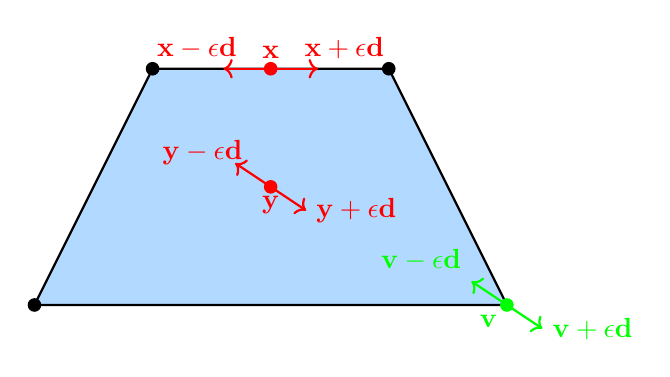
\begin{tikzpicture}[scale=1.5]
    % Draw the polytope
    \fill[blue!50!cyan,opacity=0.3] (0,0) -- (1,2) -- (3,2) -- (4,0) -- cycle;

    % Draw the edges of the polytope
    \draw[thick] (0,0) -- (1,2) -- (3,2) -- (4,0) -- cycle;

    % Label vertices
    \filldraw[black] (0,0) circle (1.5pt);
    \filldraw[black] (1,2) circle (1.5pt);
    \filldraw[black] (3,2) circle (1.5pt);
    \filldraw[green] (4,0) circle (1.5pt) node[below left] {$\mathbf{v}$};

    % Mark the point x on the edge
    \filldraw[red] (2,2) circle (1.5pt) node[above] {$\mathbf{x}$};

    % Draw the perturbation directions on the edge
    \draw[->, thick, red] (2,2) -- (2.4,2) node[midway, above right] {$\mathbf{x} + \epsilon \mathbf{d}$};
    \draw[->, thick, red] (2,2) -- (1.6,2) node[midway, above left] {$\mathbf{x} - \epsilon \mathbf{d}$};

    % Mark another point inside the polytope
    \filldraw[red] (2,1) circle (1.5pt) node[below] {$\mathbf{y}$};

    % Draw the perturbation directions inside the polytope
    \draw[->, thick, red] (2,1) -- (2.3,0.8) node[right] {$\mathbf{y} + \epsilon \mathbf{d}$};
    \draw[->, thick, red] (2,1) -- (1.7,1.2) node[midway, above left] {$\mathbf{y} - \epsilon \mathbf{d}$};

    % Draw perturbation directions for the green vertex
    \draw[->, thick, green] (4,0) -- (4.3,-0.2) node[right] {$\mathbf{v} + \epsilon \mathbf{d}$};
    \draw[->, thick, green] (4,0) -- (3.7,0.2) node[above left] {$\mathbf{v} - \epsilon \mathbf{d}$};

\end{tikzpicture}
\end{document}
